\section{Game Architecture Overview}
The essential systems of the game should support the design specifications of the game which are described in section \ref{gamedesign:selectionofgametype}.
\begin{itemize}
    \item Network to support multiplayer
    \item Input System which can support keyboard and mouse input, gamepad input, and touchscreen input.
    \item Level and mission generation which creates the game world and goal of the game, and can be easily modified by users
\end{itemize}
Early prototyping was done on the essential systems to find 3rd party APIs alongside Unity3D, that would speed up the development of these systems.
With these main systems in mind we can set up the lower-middle layer of the diagram.
By prioritising the implementation of lower layers such as \textit{Network, Input, AI} and \textit{Level generation}, we form a base onto which we implement more game-specific layers above them.

\begin{figure}
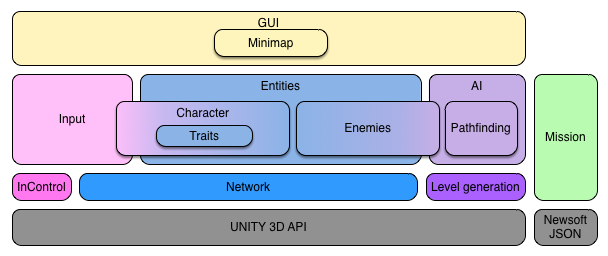
\includegraphics[width = \textwidth]{figures/architecture/game_architecture_overview.png}
\end{figure}

The network has to handle the enemies and characters in the game such that they can be synchronised with all the players, handled in the Entity structure above the network level.
Furthermore, these characters should be connected to the input system as they are to be controlled by players.

Enemies are not controlled by players but are AI's in the game and have a specific behaviour.
The way they are moving throughout the map should be controlled by some AI system which is created from the output of the level generator.

The GUI layer encapsulates all components related to views in the game.

All components will be described in greater detail later in this part of the report.

The input layer handles different input sources such as a touchscreen, gamepads, keyboard and mouse.

The level generation layer is responsible instantiating the game world according to level and mission chosen by the player.
